There are several papers that we would like to mention developing the topics related to the present work. Yoshua Bengio, Aaron Courville, and Pascal Vincent review representation learning and why it is important, single layer and deep models, autoencoders, as well as other related architectures for deep learning \cite{bengio2012rep}. For further elaboration on stacked autoencoders (and more specifically denoising autoencoders) we refer the reader to \cite{vincent2010stacked}. Hinton et al. describe in \cite{hinton2006learning} how to successfully train deep multilayer networks, like the stacked autoencoder we use in this paper. The theory and methods behind the backpropagation algorithm, a variant of SGD designed for neural networks, that we use is classic and can be found in \cite{hecht1989theory,bottou-91c}. Future plans include using a genetic algorithm (GA) to train the autoencoder instead of backpropagation. A survey of GAs and how they perform optimization can be found in \cite{srinivas1994genetic}. Cant{\'u}-Paz discusses parallel GAs, which will be essential to efficiently training our autoencoder \cite{cantu1998survey}.

\begin{figure}[h]
\centering
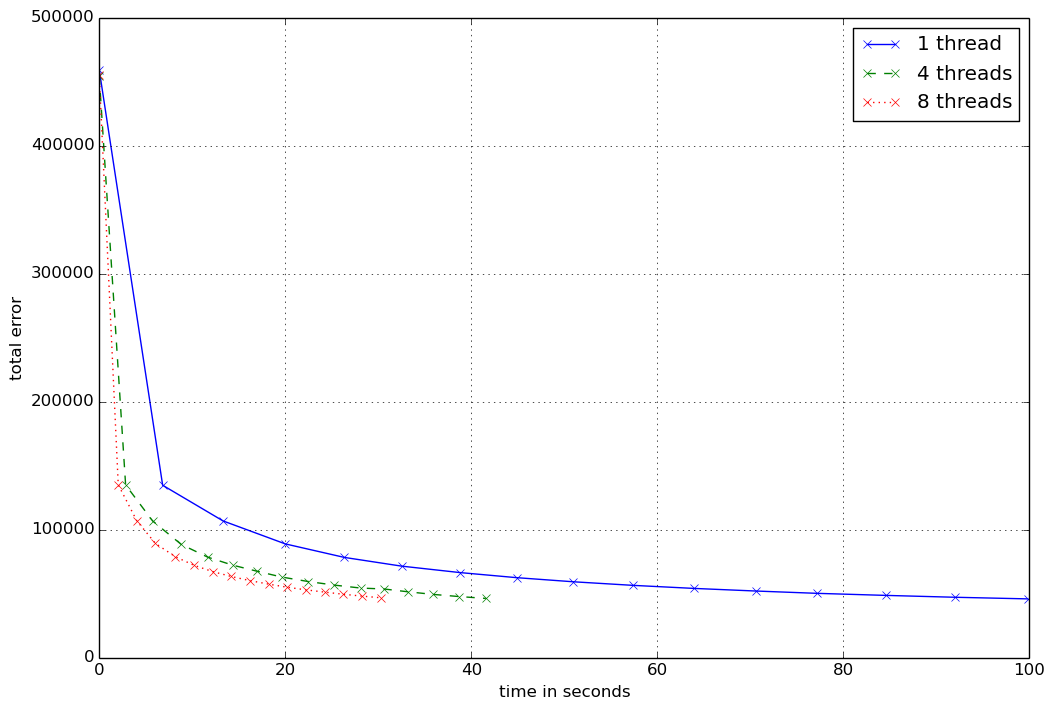
\includegraphics[width=1.0\linewidth]{experiment1.png}
\caption{Performance results on a single autoencoder layer with 500 hidden nodes and trained for 15 iterations. Plot shows time elapsed versus total training error over 5000 images for 1, 4, and 8 threads.}
\label{fig:experiment1}
\end{figure}

